%% Recombination rate coefficients in EXHALE: H I, He I, He II, He I 2^3 S
%% Comparison with Draine 2011, Verner&Ferland 1996, Benjamin+1999, and
%% the recent escape model of Taylor et al. 2025; status of newer data.
%% Author: Kwang-Il Seon
\documentclass[english,a4paper]{kiseon_memo}
\synctex=1
\usepackage{graphicx}
\usepackage{booktabs}
\usepackage{amsmath,amssymb}
\usepackage{listings}
\usepackage{xcolor}
\usepackage{babel}
\setlength{\emergencystretch}{3em}
\lstset{basicstyle=\ttfamily\footnotesize,frame=single,breaklines=true,
        numbers=left,numberstyle=\tiny\color{gray},language=Python}

\newcommand{\acm}{\ensuremath{\,\mathrm{cm^3\,s^{-1}}}}

\begin{document}

\title{Recombination Rate Coefficients in EXHALE:\\
H\,I, He\,I, He\,II, and the He\,I\,$2^3$S Triplet,\\
with Benchmarks and the Status of Newer Data}
\author{Kwang-Il Seon}
\date{2026-06-30}
\maketitle

\tableofcontents
\bigskip

%=============================================================================
\section{Overview}
%=============================================================================

This memo documents how EXHALE treats recombination onto H\,I, He\,I,
He\,II, and the metastable He\,I\,$2^3$S level (the lower level of the
He\,10830 line), benchmarks the adopted coefficients against other
published fits, and reviews whether more recent data warrant an update.
The companion to this is the photoionization cross-section memo
(\texttt{photoion\_cross\_sections.tex}); together they cover the two
microphysical inputs that set the H/He ionization balance and the
He\,$2^3$S population.

The two headline conclusions are: (i) EXHALE's H/He \emph{case-B}
coefficients (Hui \& Gnedin 1997) agree with the Draine (2011) case-B
fits to $\sim$$2\%$ over $5\times10^3$--$2\times10^4\,$K --- they are not
outdated; the larger differences seen against some escape codes are the
\emph{case-A vs.\ case-B} modeling choice, not data vintage. (ii) EXHALE's
He\,$2^3$S triplet recombination (Benjamin, Skillman \& Smits 1999, as
parametrized by Oklopcic \& Hirata 2018) is \emph{identical} to that
adopted by the most recent multi-species escape model (Taylor et al.\
2025), so it reflects current escape-community practice.

%=============================================================================
\section{What EXHALE uses}\label{sec:exhale}
%=============================================================================

All H/He recombination coefficients are defined in
\texttt{src/modules/radiation/Cool\_coeff.f90} and assembled in
\texttt{ionization\_equilibrium.f90}. Units are \acm{}.

\paragraph{H\,II $\to$ H\,I and He\,III $\to$ He\,II (Hui \& Gnedin 1997,
case B).} With $\lambda_i = 2 T_i/T$ and $T_i$ the ionization temperature
($157807,\ 285335,\ 631515\,$K for H\,I, He\,I, He\,II),
\begin{align}
\alpha_{\rm H\,II}^{B}(T) &= 2.753\times10^{-14}\,
   \frac{\lambda_{\rm H}^{1.5}}{[1+(\lambda_{\rm H}/2.74)^{0.407}]^{2.242}}, \\
\alpha_{\rm He\,III}^{B}(T) &= 2\times 2.753\times10^{-14}\,
   \frac{\lambda_{\rm He^+}^{1.5}}{[1+(\lambda_{\rm He^+}/2.74)^{0.407}]^{2.242}},
\end{align}
the second being the hydrogenic ($Z=2$) scaling of the first. Case B (the
``on-the-spot'' approximation) excludes direct recombination to the
ground state, whose re-emitted photon is assumed re-absorbed locally.

\paragraph{He\,II $\to$ He\,I (two regimes).} When the He\,$2^3$S network
is \emph{off}, EXHALE uses the Hui \& Gnedin (1997) total case-B
coefficient $\alpha_{\rm He\,II}^{B}=1.26\times10^{-14}\,\lambda_{\rm He}^{0.75}$.
When the network is \emph{on}, the He\,II$\to$He\,I recombination is split
into singlet and triplet channels (\texttt{ionization\_equilibrium.f90};
the total case-B value is overwritten), following Benjamin, Skillman \&
Smits (1999) as parametrized by Oklopcic \& Hirata (2018):
\begin{align}
\alpha_{1}(T) &= 1.54\times10^{-13}\,(T/10^4)^{-0.486}
   \qquad(\text{singlet, }1^1S),\\
\alpha_{3}(T) &= 2.10\times10^{-13}\,(T/10^4)^{-0.778}
   \qquad(\text{triplet, }2^3S).
\end{align}
These are \emph{effective} (cascade-summed) coefficients: $\alpha_3$ is
the total rate at which recombinations populate the metastable $2^3S$
level via direct capture plus radiative cascades through the higher
triplet terms. The triplet captures the majority of He recombinations,
$\alpha_3/(\alpha_1+\alpha_3)\simeq0.53$--$0.63$ over
$5\times10^3$--$2\times10^4\,$K (Table~\ref{tab:he}).

Metals use the modern Badnell radiative + dielectronic recombination
(RR$+$DR), described in the cooling memo, and are not revisited here.

%=============================================================================
\section{H$^+\to$ H: case-A vs.\ case-B, not data vintage}\label{sec:H}
%=============================================================================

Figure~\ref{fig:recH} and Table~\ref{tab:H} compare EXHALE's case-B
$\alpha_{\rm H\,II}$ with the Draine (2011) case-A/B fits and with the
total (case-A) coefficient adopted by the recent escape model of Taylor
et al.\ (2025, their Storey \& Hummer 1995 value). EXHALE tracks the
Draine \emph{case-B} curve to $\sim$$2\%$ across the whole range. The
Taylor+2025 value is $\sim$$40$--$90\%$ higher, but that is because it is
a \emph{case-A} (total) rate: codes that transport the diffuse
recombination continuum explicitly use case A, whereas EXHALE's
on-the-spot scheme correctly uses case B. The underlying data agree; the
difference is the radiative-transfer treatment.

\begin{table}[h]
\centering
\caption{H$^+\to$H recombination coefficient ($10^{-13}\acm$).}
\label{tab:H}
\begin{tabular}{rrrrr}
\toprule
$T$ [K] & EXHALE (B) & Draine (B) & Draine (A) & Taylor+25 (A)\\
\midrule
5000  & 4.543 & 4.428 & 6.733 & 6.608\\
10000 & 2.592 & 2.540 & 4.130 & 4.241\\
15000 & 1.837 & 1.818 & 3.087 & 3.271\\
20000 & 1.428 & 1.428 & 2.505 & 2.721\\
\bottomrule
\end{tabular}
\end{table}

\begin{figure}[h]
\centering
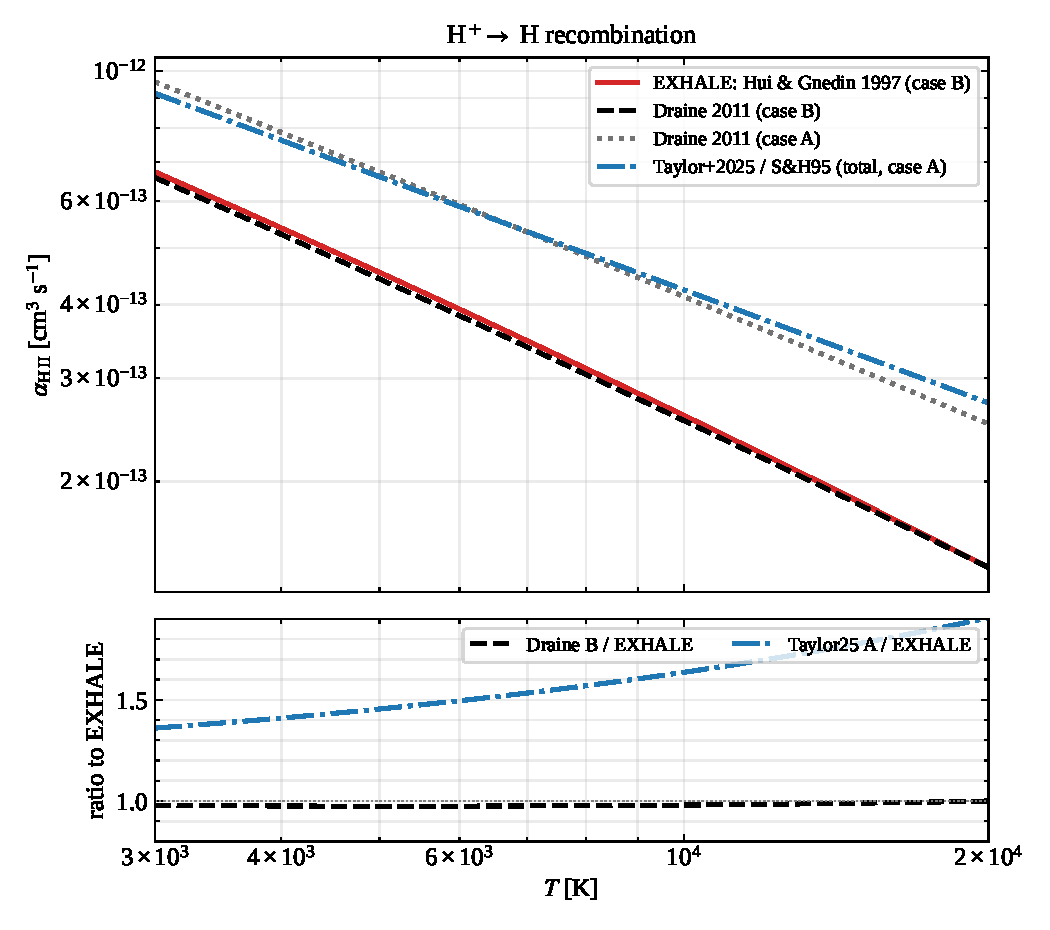
\includegraphics[width=0.72\textwidth]{figures/rec_H.pdf}
\caption{H$^+\to$H recombination. EXHALE (Hui \& Gnedin 1997, case B; red)
overlaps the Draine (2011) case-B fit to $\sim$2\% (bottom panel); the
case-A (total) curves of Draine and Taylor+2025 are $\sim$40--90\% higher.
The offset is the case-A vs.\ case-B choice, not a data update.}
\label{fig:recH}
\end{figure}

%=============================================================================
\section{Helium recombination}\label{sec:He}
%=============================================================================

The left panel of Fig.~\ref{fig:recHe} repeats the case-A/B story for
He$^{++}\to$He$^+$: EXHALE (case B) matches the hydrogenic Draine case-B
to $\sim$2\%, while the Verner \& Ferland (1996) total used by Taylor+2025
is $\sim$45\% higher (case A). The right panel shows He$^+\to$He: the Hui
\& Gnedin total case-B, and the Benjamin+1999 singlet/triplet split that
EXHALE uses when the $2^3S$ network is active. Table~\ref{tab:he} lists
the values.

Two points are worth noting. (i) The triplet recombination $\alpha_3$
(the quantity that feeds He\,10830) is \emph{identical} in EXHALE and in
the latest escape models --- both adopt Benjamin+1999. (ii) The
Benjamin+1999 effective total $\alpha_1+\alpha_3$ is $\sim$40\% larger
than the Hui \& Gnedin (1997) total case-B (e.g.\ $3.64$ vs.\
$2.62\times10^{-13}\acm$ at $10^4\,$K); the two come from different methods
(effective level-resolved cascade sums vs.\ a recombination-spectrum
case-B total). When the $2^3S$ network is on, EXHALE consistently uses the
Benjamin split for both channels, so the He ionization balance and the
metastable source term are computed from the same data set.

\begin{table}[h]
\centering
\caption{He recombination coefficients ($10^{-13}\acm$). Left: He$^{++}\to$
He$^+$. Right: He$^+\to$He --- Hui \& Gnedin total (case B) and the
Benjamin+1999 singlet $\alpha_1$, triplet $\alpha_3$, and triplet fraction.}
\label{tab:he}
\begin{tabular}{r rrr r rrrr}
\toprule
 & \multicolumn{3}{c}{He$^{++}\to$He$^+$} & & \multicolumn{4}{c}{He$^+\to$He}\\
\cmidrule(lr){2-4}\cmidrule(lr){6-9}
$T$ [K] & EXHALE(B) & Draine(B) & Tayl25(A) & & HG97 tot & $\alpha_1$ & $\alpha_3$ & $\alpha_3/(\alpha_1{+}\alpha_3)$\\
\midrule
5000  & 25.61 & 25.35 & 34.51 & & 4.400 & 2.157 & 3.601 & 0.625\\
10000 & 15.45 & 15.13 & 22.61 & & 2.616 & 1.540 & 2.100 & 0.577\\
15000 & 11.37 & 11.09 & 17.66 & & 1.930 & 1.265 & 1.532 & 0.548\\
20000 &  9.09 &  8.86 & 14.82 & & 1.556 & 1.100 & 1.225 & 0.527\\
\bottomrule
\end{tabular}
\end{table}

\begin{figure}[h]
\centering
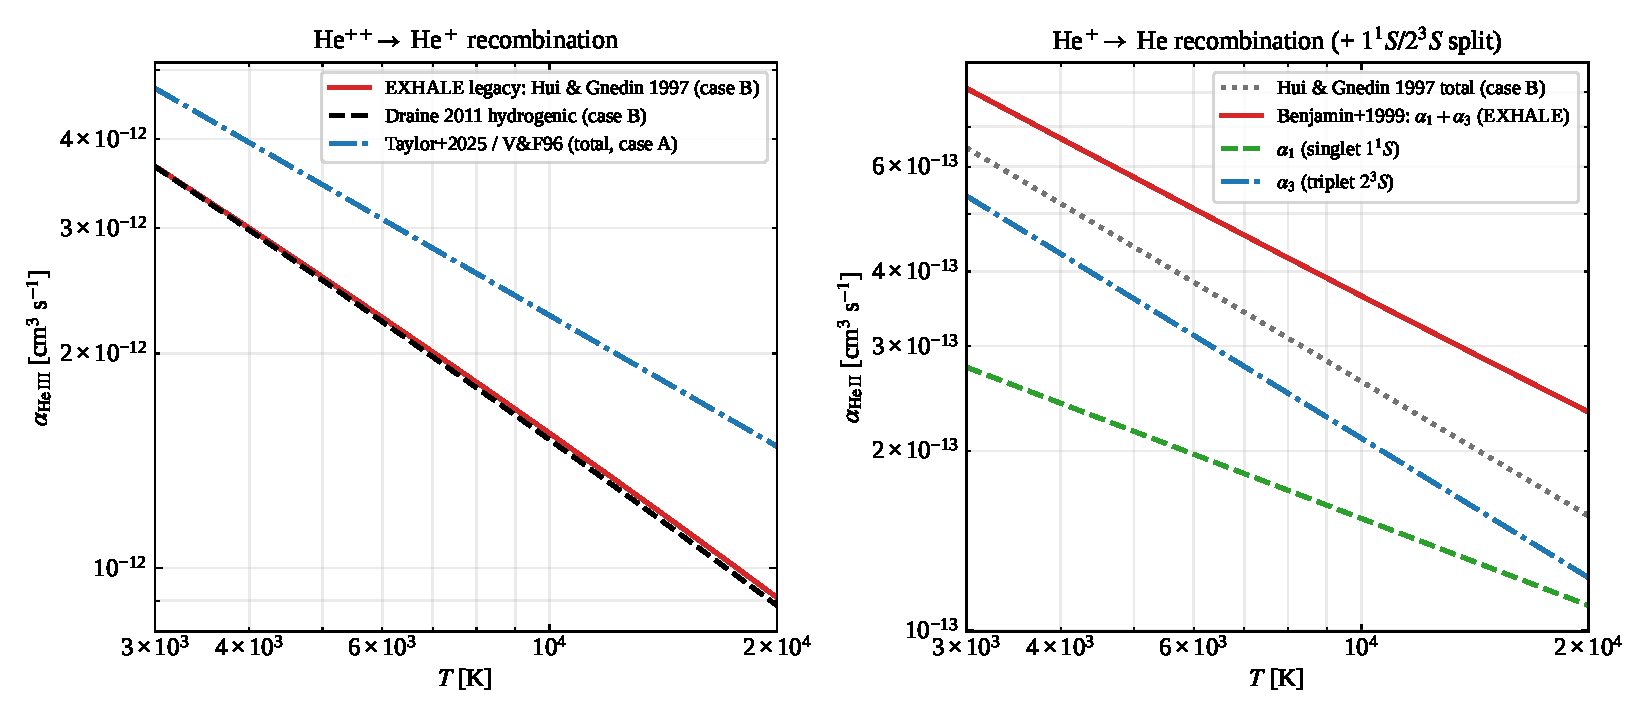
\includegraphics[width=0.98\textwidth]{figures/rec_He.pdf}
\caption{Helium recombination. \textbf{Left:} He$^{++}\to$He$^+$ ---
EXHALE case B (red) $\approx$ Draine hydrogenic case B (black); Verner \&
Ferland 1996 / Taylor+2025 total (case A) is $\sim$45\% higher.
\textbf{Right:} He$^+\to$He --- Hui \& Gnedin total case B (dotted) and the
Benjamin+1999 singlet/triplet split ($\alpha_1+\alpha_3$, $\alpha_1$,
$\alpha_3$) used by EXHALE when the $2^3S$ network is active.}
\label{fig:recHe}
\end{figure}

%=============================================================================
\section{Is there newer data?}\label{sec:newer}
%=============================================================================

\paragraph{H\,I and He\,II (hydrogenic).} Essentially solved. Hui \&
Gnedin (1997), Storey \& Hummer (1995), Verner \& Ferland (1996), and
Badnell (2006) agree to $\sim$1--2\% (Fig.~\ref{fig:recH}). No update is
warranted; the only meaningful choice is case A vs.\ B (\S\ref{sec:H}).

\paragraph{He\,I total and the $2^3S$ triplet --- no update available.}
The newer He\,I references often cited here --- \textbf{Porter, Ferland,
Storey \& Detisch (2012, MNRAS 425, L28; 2013 erratum MNRAS 433, L89)}
(the Cloudy default) and \textbf{Del Zanna \& Storey (2022)} --- are
\emph{emissivity} papers. They improve the He\,I \emph{line cascade /
line-ratio} predictions, but they do \emph{not} provide, and do not
change, the quantity EXHALE needs: the \emph{total} (effective)
recombination into the triplet ladder, $\alpha_3$, which all funnels to
the metastable $2^3S$. That total is set by (case-B total recombination)
$\times$ (triplet spin fraction $3/4$) --- ultimately by the
photoionization cross sections (Milne) and spin statistics --- and is
\emph{robust} across modern treatments:
\begin{itemize}
\item EXHALE (Benjamin+1999):
  $\alpha_3 = 2.10\times10^{-13}T_4^{-0.778}$,
  $\alpha_1 = 1.54\times10^{-13}T_4^{-0.486}\acm$;
\item 2025 thermosphere model (arXiv:2509.14499; from
  Draine 2011 \S14.3): $\alpha_3 = \tfrac34\,(2.72\times10^{-13}T_4^{-0.789})
  = 2.04\times10^{-13}T_4^{-0.789}$, with the \emph{identical} singlet
  $\alpha_1 = 1.54\times10^{-13}T_4^{-0.486}\acm$.
\end{itemize}
$\alpha_3$ agrees to $\sim$2--3\% and $\alpha_1$ is identical. The most
recent multi-species escape model (Taylor et al.\ 2025) likewise adopts
Benjamin+1999 for the triplet. Attempting to extract a different value
from the local Cloudy install confirmed the point: its
\texttt{he\_iso\_recomb.dat} stores the direct radiative
recombination for each level, and summing all triplet ($S=3$) captures \emph{is} the
effective $\alpha(2^3S)$ in case B, but the file carries no usable
level$\to(n,\ell,S)$ map for its $1642$ He levels (only $111$ are resolved
in \texttt{helike\_energies.dat}) and a trial sum overshoots the known
case-A total by $\sim$2$\times$ --- i.e.\ there is no clean drop-in Cloudy
number either.

\paragraph{Recommendation.} \textbf{Leave the recombination as it is.}
EXHALE's Benjamin+1999 $\alpha_1,\alpha_3$ already match the latest
escape-modeling practice and the underlying atomic physics to
$\lesssim3\%$; the Porter/Del Zanna ``updates'' are line-emissivity
improvements that do not alter the total $2^3S$ recombination. The H/He
case-B rates likewise need no change. The single worthwhile atomic-data
update in this round is the \emph{photoionization} of the He\,I ground
state (Verner+1996, now the EXHALE default; see
\texttt{docs/Update\_EXHALE} \S22), which shifts the He\,10830 depth by
$\sim$3\%.

%=============================================================================
\section{Reproducing this comparison}\label{sec:script}
%=============================================================================

\begin{verbatim}
cd ATES/EXHALE/docs
python3 compare_recombination.py
# -> figures/rec_H.pdf, figures/rec_He.pdf
\end{verbatim}

The script ports the EXHALE coefficients from \texttt{Cool\_coeff.f90}
verbatim and codes the Draine (2011), Verner \& Ferland (1996) /
Taylor+2025, and Benjamin+1999 reference fits.

\end{document}
